\documentclass[12pt,]{article}
\usepackage{lmodern}
\usepackage{amssymb,amsmath}
\usepackage{ifxetex,ifluatex}
\usepackage{fixltx2e} % provides \textsubscript
\ifnum 0\ifxetex 1\fi\ifluatex 1\fi=0 % if pdftex
  \usepackage[T1]{fontenc}
  \usepackage[utf8]{inputenc}
\else % if luatex or xelatex
  \ifxetex
    \usepackage{mathspec}
  \else
    \usepackage{fontspec}
  \fi
  \defaultfontfeatures{Ligatures=TeX,Scale=MatchLowercase}
\fi
% use upquote if available, for straight quotes in verbatim environments
\IfFileExists{upquote.sty}{\usepackage{upquote}}{}
% use microtype if available
\IfFileExists{microtype.sty}{%
\usepackage{microtype}
\UseMicrotypeSet[protrusion]{basicmath} % disable protrusion for tt fonts
}{}
\usepackage[margin=1in]{geometry}
\usepackage{hyperref}
\hypersetup{unicode=true,
            pdftitle={STAT 6910: HW 8},
            pdfauthor={David Angeles},
            pdfborder={0 0 0},
            breaklinks=true}
\urlstyle{same}  % don't use monospace font for urls
\usepackage{color}
\usepackage{fancyvrb}
\newcommand{\VerbBar}{|}
\newcommand{\VERB}{\Verb[commandchars=\\\{\}]}
\DefineVerbatimEnvironment{Highlighting}{Verbatim}{commandchars=\\\{\}}
% Add ',fontsize=\small' for more characters per line
\usepackage{framed}
\definecolor{shadecolor}{RGB}{248,248,248}
\newenvironment{Shaded}{\begin{snugshade}}{\end{snugshade}}
\newcommand{\KeywordTok}[1]{\textcolor[rgb]{0.13,0.29,0.53}{\textbf{#1}}}
\newcommand{\DataTypeTok}[1]{\textcolor[rgb]{0.13,0.29,0.53}{#1}}
\newcommand{\DecValTok}[1]{\textcolor[rgb]{0.00,0.00,0.81}{#1}}
\newcommand{\BaseNTok}[1]{\textcolor[rgb]{0.00,0.00,0.81}{#1}}
\newcommand{\FloatTok}[1]{\textcolor[rgb]{0.00,0.00,0.81}{#1}}
\newcommand{\ConstantTok}[1]{\textcolor[rgb]{0.00,0.00,0.00}{#1}}
\newcommand{\CharTok}[1]{\textcolor[rgb]{0.31,0.60,0.02}{#1}}
\newcommand{\SpecialCharTok}[1]{\textcolor[rgb]{0.00,0.00,0.00}{#1}}
\newcommand{\StringTok}[1]{\textcolor[rgb]{0.31,0.60,0.02}{#1}}
\newcommand{\VerbatimStringTok}[1]{\textcolor[rgb]{0.31,0.60,0.02}{#1}}
\newcommand{\SpecialStringTok}[1]{\textcolor[rgb]{0.31,0.60,0.02}{#1}}
\newcommand{\ImportTok}[1]{#1}
\newcommand{\CommentTok}[1]{\textcolor[rgb]{0.56,0.35,0.01}{\textit{#1}}}
\newcommand{\DocumentationTok}[1]{\textcolor[rgb]{0.56,0.35,0.01}{\textbf{\textit{#1}}}}
\newcommand{\AnnotationTok}[1]{\textcolor[rgb]{0.56,0.35,0.01}{\textbf{\textit{#1}}}}
\newcommand{\CommentVarTok}[1]{\textcolor[rgb]{0.56,0.35,0.01}{\textbf{\textit{#1}}}}
\newcommand{\OtherTok}[1]{\textcolor[rgb]{0.56,0.35,0.01}{#1}}
\newcommand{\FunctionTok}[1]{\textcolor[rgb]{0.00,0.00,0.00}{#1}}
\newcommand{\VariableTok}[1]{\textcolor[rgb]{0.00,0.00,0.00}{#1}}
\newcommand{\ControlFlowTok}[1]{\textcolor[rgb]{0.13,0.29,0.53}{\textbf{#1}}}
\newcommand{\OperatorTok}[1]{\textcolor[rgb]{0.81,0.36,0.00}{\textbf{#1}}}
\newcommand{\BuiltInTok}[1]{#1}
\newcommand{\ExtensionTok}[1]{#1}
\newcommand{\PreprocessorTok}[1]{\textcolor[rgb]{0.56,0.35,0.01}{\textit{#1}}}
\newcommand{\AttributeTok}[1]{\textcolor[rgb]{0.77,0.63,0.00}{#1}}
\newcommand{\RegionMarkerTok}[1]{#1}
\newcommand{\InformationTok}[1]{\textcolor[rgb]{0.56,0.35,0.01}{\textbf{\textit{#1}}}}
\newcommand{\WarningTok}[1]{\textcolor[rgb]{0.56,0.35,0.01}{\textbf{\textit{#1}}}}
\newcommand{\AlertTok}[1]{\textcolor[rgb]{0.94,0.16,0.16}{#1}}
\newcommand{\ErrorTok}[1]{\textcolor[rgb]{0.64,0.00,0.00}{\textbf{#1}}}
\newcommand{\NormalTok}[1]{#1}
\usepackage{graphicx,grffile}
\makeatletter
\def\maxwidth{\ifdim\Gin@nat@width>\linewidth\linewidth\else\Gin@nat@width\fi}
\def\maxheight{\ifdim\Gin@nat@height>\textheight\textheight\else\Gin@nat@height\fi}
\makeatother
% Scale images if necessary, so that they will not overflow the page
% margins by default, and it is still possible to overwrite the defaults
% using explicit options in \includegraphics[width, height, ...]{}
\setkeys{Gin}{width=\maxwidth,height=\maxheight,keepaspectratio}
\IfFileExists{parskip.sty}{%
\usepackage{parskip}
}{% else
\setlength{\parindent}{0pt}
\setlength{\parskip}{6pt plus 2pt minus 1pt}
}
\setlength{\emergencystretch}{3em}  % prevent overfull lines
\providecommand{\tightlist}{%
  \setlength{\itemsep}{0pt}\setlength{\parskip}{0pt}}
\setcounter{secnumdepth}{0}
% Redefines (sub)paragraphs to behave more like sections
\ifx\paragraph\undefined\else
\let\oldparagraph\paragraph
\renewcommand{\paragraph}[1]{\oldparagraph{#1}\mbox{}}
\fi
\ifx\subparagraph\undefined\else
\let\oldsubparagraph\subparagraph
\renewcommand{\subparagraph}[1]{\oldsubparagraph{#1}\mbox{}}
\fi

%%% Use protect on footnotes to avoid problems with footnotes in titles
\let\rmarkdownfootnote\footnote%
\def\footnote{\protect\rmarkdownfootnote}

%%% Change title format to be more compact
\usepackage{titling}

% Create subtitle command for use in maketitle
\newcommand{\subtitle}[1]{
  \posttitle{
    \begin{center}\large#1\end{center}
    }
}

\setlength{\droptitle}{-2em}

  \title{STAT 6910: HW 8}
    \pretitle{\vspace{\droptitle}\centering\huge}
  \posttitle{\par}
    \author{David Angeles}
    \preauthor{\centering\large\emph}
  \postauthor{\par}
    \date{}
    \predate{}\postdate{}
  

\begin{document}
\maketitle

\begin{verbatim}
## Warning: package 'emmeans' was built under R version 3.4.4
\end{verbatim}

\begin{verbatim}
## NOTE: As of emmeans versions > 1.2.3,
##       The 'cld' function will be deprecated in favor of 'CLD'.
##       You may use 'cld' only if you have package:multcomp attached.
\end{verbatim}

\begin{verbatim}
## Warning: package 'dae' was built under R version 3.4.4
\end{verbatim}

\begin{verbatim}
## Loading required package: ggplot2
\end{verbatim}

\begin{verbatim}
## Warning: package 'ggplot2' was built under R version 3.4.4
\end{verbatim}

\subsection{Problem 1 (6 in text)}\label{problem-1-6-in-text}

The purpose of the experiment run by M. Weber, R. Zielinski, J. Y. Lee,
S. Xia, and Y. Guo in 2010 was to determine the best way to heat 3 cups
of water (for preparation of boxed meals) to \(90^o\)F on a kitchen
stove as qsuickly as possible. In this experiment, only one stove was
used, and the three treatment factors were

\begin{center}
C: diameter of pot (5.5, 6.25 and 8.625 inches; coded 1, 2, 3)\\
D: burner size (small, large; coded 1, 2)\\
E: cover (no, yes; coded 1, 2).
\end{center}

\textbf{(b)} A pilot experiment suggested that the error variance
\(\sigma^2\) would be no larger than 318.9 sec\(^2\). The experimenters
wanted to be able to test the hypothesis of no differences in the
effects of heating time due to the 12 treatments, with a probability of
0.9 of rejecting the hypothesis if the true difference was
\(\Delta= 60\) secs. The test was to be done at level \(\alpha = 0.05\).
Calculate the number of observations that should be taken on each of the
12 treatments.

(In Part (b), either follow the instructions in Chapter 3 (ignoring
blocking) or follow the instructions in Section 10.6.3, which are quite
similar, assuming b = 4 blocks.)

\textbf{solution}

\begin{Shaded}
\begin{Highlighting}[]
\NormalTok{v =}\StringTok{ }\DecValTok{12}\NormalTok{; sig2 =}\StringTok{ }\FloatTok{318.9}\NormalTok{; alpha =}\StringTok{ }\FloatTok{0.05}\NormalTok{; pwr =}\StringTok{ }\FloatTok{0.90}\NormalTok{; del =}\StringTok{ }\KeywordTok{c}\NormalTok{(}\DecValTok{60}\NormalTok{); list_of_size <-}\StringTok{ }\OtherTok{NULL}
\ControlFlowTok{for}\NormalTok{ (i }\ControlFlowTok{in} \DecValTok{1}\NormalTok{) \{delta <-}\StringTok{ }\NormalTok{del[i]}
\NormalTok{x<-}\StringTok{ }\KeywordTok{pwr.anova.test}\NormalTok{(}\DataTypeTok{k =}\NormalTok{ v, }\DataTypeTok{sig.level =}\NormalTok{ alpha , }\DataTypeTok{power =}\NormalTok{ pwr ,}
\DataTypeTok{f =} \KeywordTok{sqrt}\NormalTok{(delta}\OperatorTok{^}\DecValTok{2}\OperatorTok{/}\NormalTok{(}\DecValTok{2}\OperatorTok{*}\NormalTok{v}\OperatorTok{*}\NormalTok{sig2)))}
\NormalTok{list_of_size <-}\StringTok{ }\KeywordTok{c}\NormalTok{(list_of_size, x}\OperatorTok{$}\NormalTok{n)}
\NormalTok{\}}
\NormalTok{list_of_size}
\end{Highlighting}
\end{Shaded}

\begin{verbatim}
## [1] 4.643032
\end{verbatim}

If we ignore blocking and use \(\sigma^2 = 318.9\), \(\Delta = 60\),
\(v=12\), \(\pi = .90\), and an \(\alpha\)-level of \(\alpha =.05\) we
get that the sample size needd in \(5\).

\textbf{(c)}

The experimenters ultimately decided that they would use a randomized
complete block design with \(b = 4\) blocks for the experiment, where
each block was defined by experimenter and day. The data are shown in
Table 10.20. Using the block--treatment model (10.4.1), p.~310, for a
randomized complete block design, check the assumptions on the model and
test the hypothesis of no effects on the heating time due to treatments.

(In Part (c), you may detect an outlier -- in practice you might run the
subsequent analyses with and without the outlier and include both
results, commenting on any discrepancies. For this homework, please just
proceed with the outlier still in the data set -- this may not be the
best choice, but it will make everyone's answers uniform!)

Using the block--treatment model (10.4.1) we have:

\begin{center}
$Y_{hi} = \mu + \theta_h + \tau_i + \epsilon_{hi},$\\
$\epsilon_{hi} \sim N(0,\sigma^2)$\\
$\epsilon_{hi}$'s mutually independent,\\
$h = 1,\ldots, b$; $i = 1, \ldots , v$.
\end{center}

where \(\mu\) is a constant, \(\theta_h\) is the effect of the \(h\)th
block, \(\tau_i\) is the effect of the \(i\)th treatment, \(Y_{hi}\) is
the random variable representing the measurement on the treatment \(i\)
observed in the block \(h\), and \(\epsilon_{hi}\) is the associated
random error.

\textbf{solution}\_

\begin{Shaded}
\begin{Highlighting}[]
\NormalTok{two.way_model <-}\StringTok{ }\KeywordTok{aov}\NormalTok{(time }\OperatorTok{~}\StringTok{ }\NormalTok{block}\OperatorTok{+}\NormalTok{trtmt, }\DataTypeTok{data =}\NormalTok{ water.heating)}

\NormalTok{water.heating =}\StringTok{ }\KeywordTok{within}\NormalTok{(water.heating, \{}
  \CommentTok{# Compute predicted, residual, and standardized residual values}
\NormalTok{  ypred =}\StringTok{ }\KeywordTok{fitted}\NormalTok{(two.way_model)}
\NormalTok{  e =}\StringTok{ }\KeywordTok{resid}\NormalTok{(two.way_model) }
\NormalTok{  z =}\StringTok{ }\KeywordTok{rstandard}\NormalTok{(two.way_model)}
\NormalTok{  new.code=}\StringTok{ }\KeywordTok{rep}\NormalTok{(}\DecValTok{1}\OperatorTok{:}\DecValTok{12}\NormalTok{, }\DataTypeTok{each =}\DecValTok{4}\NormalTok{)\})}
\CommentTok{# Display first 10 lines of water.heating, 4 digits per variable}
\KeywordTok{print}\NormalTok{(}\KeywordTok{head}\NormalTok{(water.heating, }\DecValTok{5}\NormalTok{), }\DataTypeTok{digits =} \DecValTok{4}\NormalTok{)}
\end{Highlighting}
\end{Shaded}

\begin{verbatim}
##   trtmt C D E block  time order new.code       z      e ypred
## 1   111 1 1 1     1 261.0     1        1 -0.9107 -35.27 296.3
## 2   111 1 1 1     2 279.0    12        1 -0.6093 -24.03 303.0
## 3   111 1 1 1     3 296.7     6        1 -0.3318 -13.09 309.8
## 4   111 1 1 1     4 282.8     5        1 -0.8712 -33.74 316.5
## 5   112 1 1 2     1 259.4    12        2 -0.9338 -36.18 295.6
\end{verbatim}

\begin{Shaded}
\begin{Highlighting}[]
\CommentTok{# Generate residual plots }
\KeywordTok{par}\NormalTok{(}\DataTypeTok{mfrow =} \KeywordTok{c}\NormalTok{(}\DecValTok{1}\NormalTok{,}\DecValTok{3}\NormalTok{))}
\KeywordTok{plot}\NormalTok{(z }\OperatorTok{~}\StringTok{ }\NormalTok{order, }\DataTypeTok{data=}\NormalTok{water.heating, }
     \DataTypeTok{main=} \StringTok{"Order vs. Std. Residuals"}\NormalTok{,}
     \DataTypeTok{ylab=}\StringTok{"Std. Residuals"}\NormalTok{, }\DataTypeTok{las=}\DecValTok{1}\NormalTok{)}
\KeywordTok{abline}\NormalTok{(}\DataTypeTok{h=}\DecValTok{0}\NormalTok{)}
\KeywordTok{plot}\NormalTok{(z }\OperatorTok{~}\StringTok{ }\NormalTok{ypred, }\DataTypeTok{data=}\NormalTok{water.heating, }
      \DataTypeTok{main=} \StringTok{"Fitted Values vs. Std. Residuals"}\NormalTok{,}
     \DataTypeTok{ylab=}\StringTok{"Std. Residuals"}\NormalTok{, }\DataTypeTok{las=}\DecValTok{1}\NormalTok{)}
\KeywordTok{abline}\NormalTok{(}\DataTypeTok{h=}\DecValTok{0}\NormalTok{)}
\KeywordTok{qqnorm}\NormalTok{(water.heating}\OperatorTok{$}\NormalTok{z)}
\CommentTok{# Line through 1st and 3rd quantile points}
\KeywordTok{qqline}\NormalTok{(water.heating}\OperatorTok{$}\NormalTok{z) }
\end{Highlighting}
\end{Shaded}

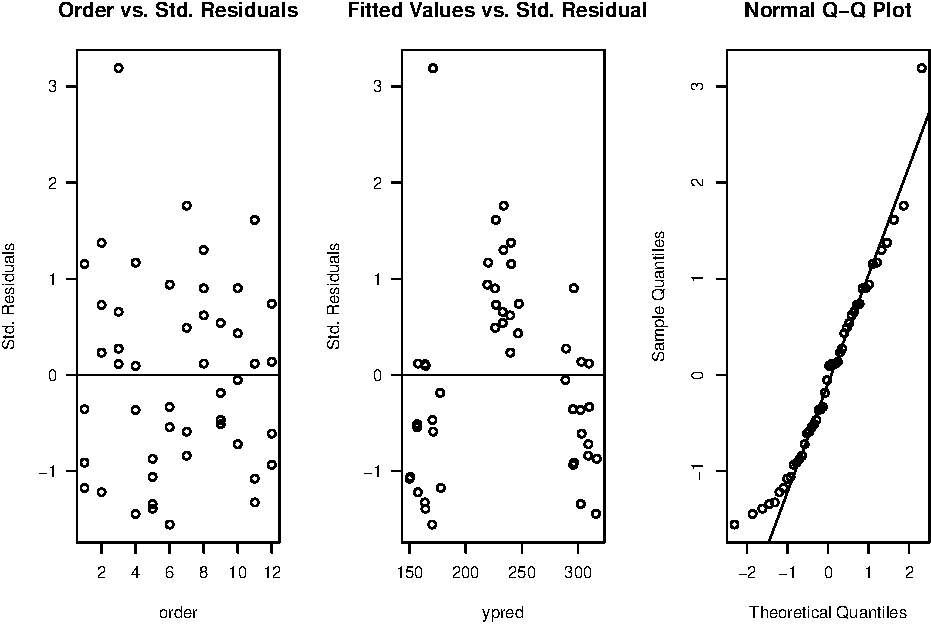
\includegraphics{Markdown_HW_8_files/figure-latex/unnamed-chunk-3-1.pdf}

Assumption (a): The error have mean 0:

\begin{Shaded}
\begin{Highlighting}[]
\KeywordTok{attach}\NormalTok{(water.heating)}
\KeywordTok{plot}\NormalTok{(z }\OperatorTok{~}\StringTok{ }\NormalTok{block, }\DataTypeTok{xaxt =} \StringTok{"n"}\NormalTok{, }\DataTypeTok{type =} \StringTok{"n"}\NormalTok{, }\DataTypeTok{xlim =} \KeywordTok{c}\NormalTok{(}\DecValTok{0}\NormalTok{, }\DecValTok{5}\NormalTok{)) }\CommentTok{# Suppress x-axis, pts}
\KeywordTok{axis}\NormalTok{(}\DecValTok{1}\NormalTok{, }\DataTypeTok{at =} \KeywordTok{c}\NormalTok{(}\DecValTok{1}\NormalTok{, }\DecValTok{2}\NormalTok{, }\DecValTok{3}\NormalTok{,}\DecValTok{4}\NormalTok{))}
\KeywordTok{points}\NormalTok{(}\DataTypeTok{x =} \KeywordTok{as.numeric}\NormalTok{(block) }\OperatorTok{+}\StringTok{ }\KeywordTok{as.numeric}\NormalTok{(new.code) }\OperatorTok{*}\StringTok{ }\FloatTok{0.05}\NormalTok{, }\DataTypeTok{y =}\NormalTok{ z,}
\DataTypeTok{pch =} \KeywordTok{as.character}\NormalTok{(}\KeywordTok{as.numeric}\NormalTok{(new.code)), }\DataTypeTok{col =} \KeywordTok{as.numeric}\NormalTok{(new.code)) }
\KeywordTok{mtext}\NormalTok{(}\StringTok{"block=0,2,4,6"}\NormalTok{, }\DataTypeTok{side =} \DecValTok{3}\NormalTok{, }\DataTypeTok{adj =} \DecValTok{1}\NormalTok{, }\DataTypeTok{line =} \DecValTok{1}\NormalTok{)}
\KeywordTok{abline}\NormalTok{(}\DataTypeTok{h =} \DecValTok{0}\NormalTok{) }\CommentTok{# Horizontal line at zero}
\end{Highlighting}
\end{Shaded}

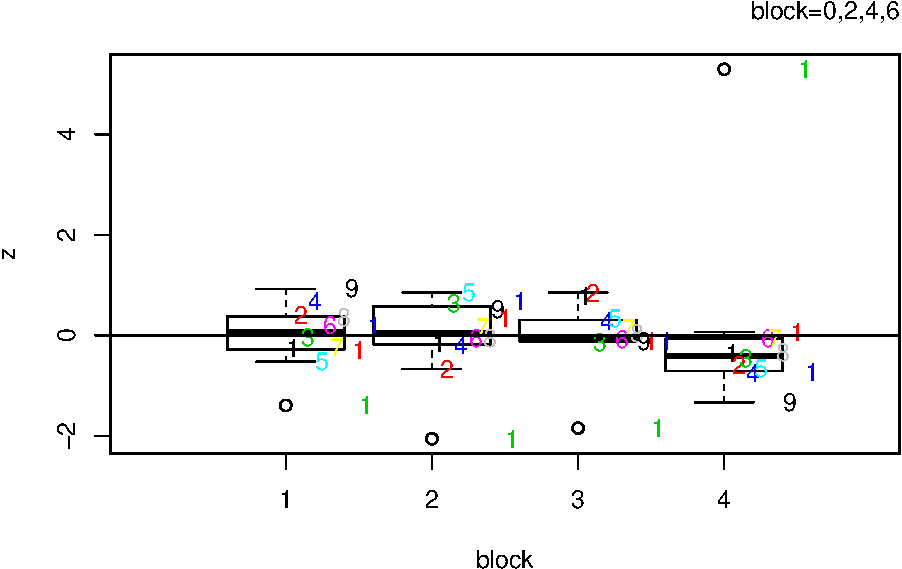
\includegraphics{Markdown_HW_8_files/figure-latex/unnamed-chunk-4-1.pdf}

\begin{Shaded}
\begin{Highlighting}[]
 \CommentTok{# Margin text, top-rt, line 1 abline(h = 0)}

\KeywordTok{interaction.plot}\NormalTok{(}\DataTypeTok{x.factor =}\NormalTok{ new.code, }\DataTypeTok{trace.factor =}\NormalTok{ block, }
                 \DataTypeTok{response=}\NormalTok{ time, }\DataTypeTok{xlab=}\StringTok{"Treatments"}\NormalTok{, }\DataTypeTok{ylab=}\StringTok{"Time"}\NormalTok{, }
                 \DataTypeTok{trace.label=}\StringTok{"Block"}\NormalTok{, }\DataTypeTok{leg.bty=}\StringTok{"b"}\NormalTok{, }\DataTypeTok{leg.bg=}\StringTok{"white"}\NormalTok{)}
\end{Highlighting}
\end{Shaded}

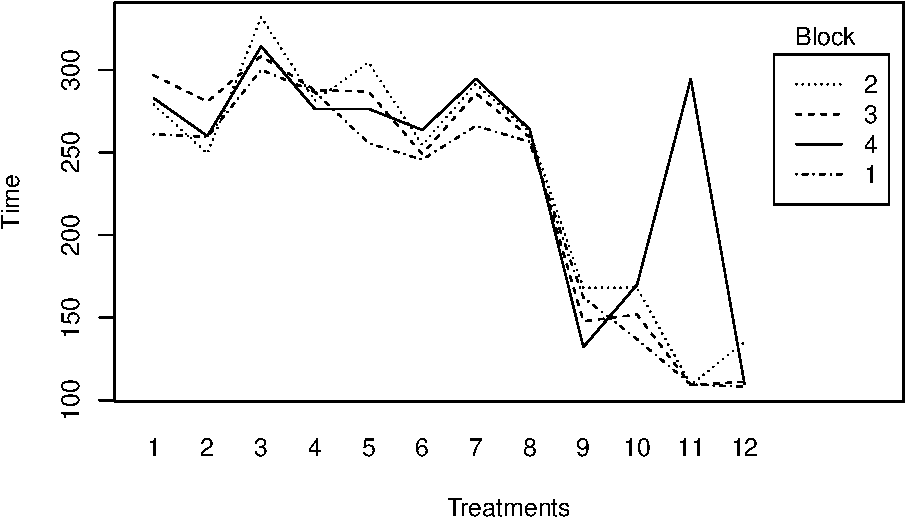
\includegraphics{Markdown_HW_8_files/figure-latex/unnamed-chunk-4-2.pdf}

Assumption (b): The error have constant variance:

By plotting the standardized residuals against the fitted values we can
see that the spread of the standardized residuals, fluctuate as the
fitted values increas. There also seems to be an outlier. The outlier
may be of interest to inspect. Hence, we can say that the equal variance
assumption is not satisfied.

Assumption (c): The error are normally distributed:

From the qq-plot above we see that the data is fairly straight. However,
there is just one apparent outliers. Therefore, the normality assumption
is fairly reasonable.

Assumption (d): The errors are independent:

From the plot of Order vs.~Std. Residuals we can see that there isn't an
apparent pattern as time increases. Therefore we feel comfortable to say
that the assumption that errors are independent is approximately
satisfies.

\begin{Shaded}
\begin{Highlighting}[]
\KeywordTok{anova}\NormalTok{(two.way_model)}
\end{Highlighting}
\end{Shaded}

\begin{verbatim}
## Analysis of Variance Table
## 
## Response: time
##           Df Sum Sq Mean Sq F value    Pr(>F)    
## block      1   2739    2739  1.6562    0.2047    
## trtmt      1 154492  154492 93.4106 1.496e-12 ***
## Residuals 45  74426    1654                      
## ---
## Signif. codes:  0 '***' 0.001 '**' 0.01 '*' 0.05 '.' 0.1 ' ' 1
\end{verbatim}

From the ANOVA table above we can see that the \(p\)-value associated
with the treatments is \(<< .05\). Therefore we can conclude that there
is some effect on the heating time due to treatments.

\textbf{(d)}

Using the factorial form of the block--treatment model similar to
(10.8.15), p.~325, but with three treatment factors, test the hypotheses
of no interactions between pairs of treatment factors, each test done at
level 0.01.

(In Part (d), the model they are asking for is still a block-treatment
model (not a block-treatment interaction model) so please use the
factorial version of the model you considered in Part (c) -- so you
should have a single term for block, but then all 2-factor and 3-factor
interactions of Factors C,D and E. You only need to evaluate the
2-factor interactions.)

\begin{Shaded}
\begin{Highlighting}[]
\NormalTok{block.trtmt.model <-}\StringTok{ }\KeywordTok{aov}\NormalTok{(time }\OperatorTok{~}\StringTok{ }\NormalTok{block}\OperatorTok{+}\StringTok{ }\NormalTok{C}\OperatorTok{*}\NormalTok{D}\OperatorTok{*}\NormalTok{E, }\DataTypeTok{data =}\NormalTok{ water.heating)}
\KeywordTok{anova}\NormalTok{(block.trtmt.model)}
\end{Highlighting}
\end{Shaded}

\begin{verbatim}
## Analysis of Variance Table
## 
## Response: time
##           Df Sum Sq Mean Sq F value    Pr(>F)    
## block      1   2739    2739  1.7396   0.19488    
## C          1 155473  155473 98.7406 3.061e-12 ***
## D          1    256     256  0.1624   0.68913    
## E          1   6080    6080  3.8611   0.05657 .  
## C:D        1   4211    4211  2.6746   0.11001    
## C:E        1     82      82  0.0518   0.82111    
## D:E        1    942     942  0.5980   0.44399    
## C:D:E      1    467     467  0.2969   0.58896    
## Residuals 39  61408    1575                      
## ---
## Signif. codes:  0 '***' 0.001 '**' 0.01 '*' 0.05 '.' 0.1 ' ' 1
\end{verbatim}

Notice from the table above that we have a single term for block and all
2-factor and 3-factor interactions of Factors C,D and E. Thus, at the
\(\alpha = .01\) level, we fail to reject test the hypotheses of no
interactions between pairs of treatment factors, since the \(p\)-value
for the interactions between C and D is \(.11\). The \(p\)-value for the
interactions between C and E is \(.82\). And the \(p\)-value for the
interactions between D and E is \(.44\).

\textbf{(e)}

Taking into account any interactions discovered in part(d), list the
contrasts that are of interest to you and, using the Scheffé method,
calculate a set of 95\% confidence intervals for the contrasts of
interest.

(For Part (e), please provide Scheffé intervals for the two main effects
contrasts in levels of C; you are certainly welcome to provide more
intervals, but these are the ones that will be graded.)

\subsection{Problem 2 (11.1 a-c)}\label{problem-2-11.1-a-c}

\textbf{(a)} For each of the three block designs in Table 11.27, draw
the connectivity graph for the design, and determine whether the design
is connected.

\begin{center}
Block Design I
\end{center}

\begin{center}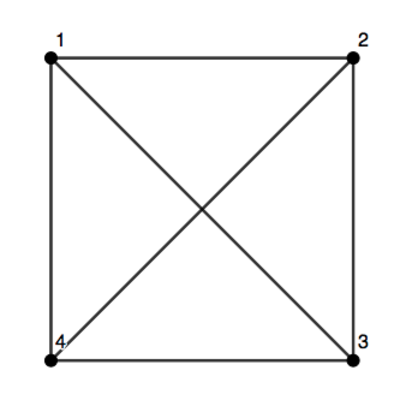
\includegraphics{Markdown_HW_8_files/figure-latex/unnamed-chunk-7-1} \end{center}

Block Design I is not connected.

\begin{center}
Block Design II
\end{center}

\begin{center}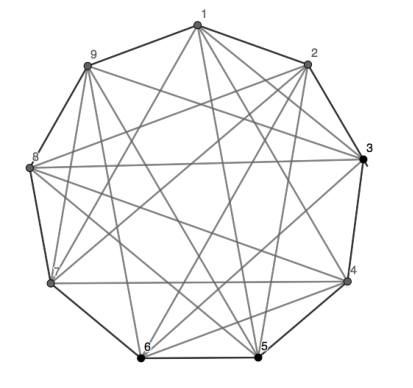
\includegraphics{Markdown_HW_8_files/figure-latex/unnamed-chunk-8-1} \end{center}

Block Design II is connected.

\begin{center}
Block Design III
\end{center}

\begin{center}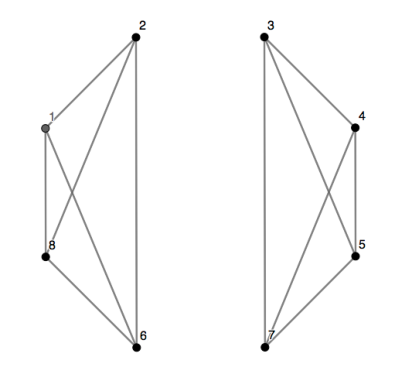
\includegraphics{Markdown_HW_8_files/figure-latex/unnamed-chunk-9-1} \end{center}

Block Design III is not connected.

\textbf{(b)} If the design is connected, determine whether or not it is
a balanced incomplete block design.

Design II is connected and we have that \(v=9\), \(b=9\), \(k=3\), and
\(r=3\). However it is not a balanced imcomplete block design by the
calculations below.

\begin{center}
$vr = 9(3) = bk \hspace{.3cm}  \checkmark$\\
$b= 9 = v \Longrightarrow b \geq v \hspace{.3cm}  \checkmark$\\
$\frac{r(k-1)}{v-1} = \frac{3(2)}{9-1} = \frac{6}{8} = \frac{3}{4} = \lambda  \notin \mathbb{Z} \Longrightarrow r(k-1) \neq \lambda (v-1)  \hspace{.3cm} \times$
\end{center}

\textbf{(c)} For designs II and III, determine graphically whether or
not \(\tau_1 - \tau_5\) and \(\tau_1 - \tau_6\) are estimable.

\textbf{solution}

Since Block Design II is connected, then all contrasts in the treatment
effects are estimable in the design. Hence \(\tau_1 - \tau_5\) and
\(\tau_1 - \tau_6\) are estimable. Futhermore, we can see that there
doesn't exist a path from 1 to 5, which means that \(\tau_1 - \tau_5\)
is not estimable. However there is a path from 1 to 6, so
\(\tau_1 - \tau_6\) is estimable.

\subsection{Problem 3 (11.5)}\label{problem-3-11.5}

In the following questions, consider an experiment to compare \(v = 7\)
treatments in blocks of size \(k = 5\).

\textbf{(a)} Show that, for this experiment, a necessary condition for a
balanced incomplete block design to exist is that \(r\) is a multiple of
5 and \(b\) is a multiple of 7.

Suppose that \(b= 7n\) for some \(n \in \mathbb{N}\) and \(r= 5m\) for
some \(m \in \mathbb{N}\).

Now we must check the three conditions needed to be an incomplete block
design:

\begin{center}
$vr = 7(5m) = 35m  \hspace{.3cm} \text{and} \hspace{.3cm} bk = (7n)5 = 35n \Longrightarrow \text{ if } n=m \hspace{.3cm}  \checkmark$\\
$b= 7n \hspace{.3cm} \text{and} \hspace{.3cm}  v=7 \Longrightarrow b \geq v \hspace{.3cm} \text{if} \hspace{.3cm} n \geq 1 \hspace{.3cm}  \checkmark$\\
$\frac{r(k-1)}{v-1} = \frac{5m(4)}{6} = \frac{20m}{6} = \frac{10m}{3}  
 \Longrightarrow  \lambda  \in \mathbb{Z} \hspace{.3cm} \text{if} \hspace{.3cm} m = 3\ell  \hspace{.3cm} \hspace{.3cm}  \checkmark$
\end{center}

So we can conclude that a necessary condition for a balanced incomplete
block design for this experiment to exist is that \(r\) is a multiple of
5 and \(b\) is a multiple of 7.

\textbf{(b)} Show that \(r\) must be at least 15.

From part (a) we see that that \(m\) must be a multiple of 3 in order
for \(\lambda \in \mathbb{Z}\). So we must have that
\(r5 (3\ell) = 15 \ell\) where \(\ell \in \mathbb{Z}\) So \(r\) must be
a multiple of 15. Next we must show that \(\ell \in \mathbb{N}\). Notice
again from part (a) that it must me true that \(n \geq1\) and \(m=n\).
So \(m\) must be psotive and therefore \(\ell \in \mathbb{N}\). Hence
\(r\) must be at least 15.

\textbf{(c)} Taking all possible combinations of five treatments from
seven gives a balanced incomplete block design with \(r = 15\).
Calculate the number of blocks that must be in this design.

Since we are still assuming \(k=5\), then we must have that \(vr = bk\),
so \(5(15) = b (5)\). Then \(b=5\). So this design must have 5 blocks.


\end{document}
